\section{Evietania - 1174051}

\subsection{Teori}
\begin{enumerate}
\item Jelaskan apa itu klasifikasi teks, sertakan gambar ilustrasi buatan sendiri.\par
klasifikasi teks adalah cara untuk memilah-milah teks berdasarkan parameter tertentu baik itu jenis teks atau jenis dari dokumen yang terdapat kumpulan teks didalamnya, sedangkan teks itu sndiri merupakan sekumpulan kata yang dapat dibaca. bisa berupa buku, majalah, rambu-rambu dan lain sebagainya.

\begin{figure}[ht]
\centering
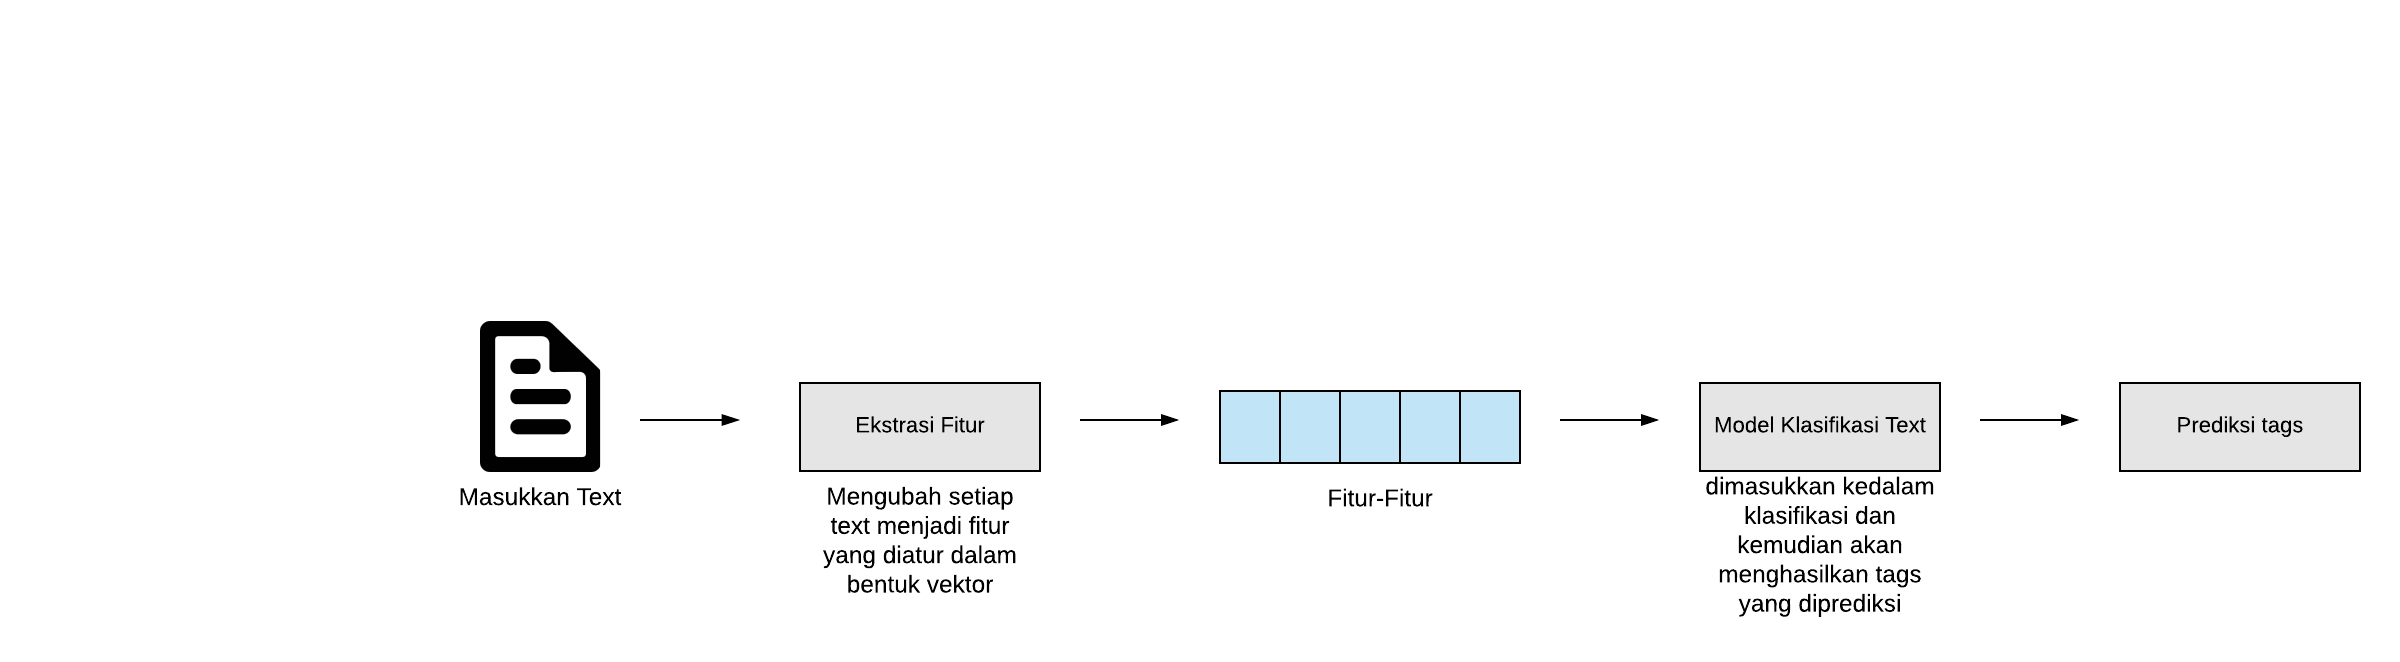
\includegraphics[scale=0.2]{figures/1174051/4/1.png}
\caption{contoh klasifikasi teks}
\label{contoh}
\end{figure}

\item Jelaskan mengapa klasifikasi bunga tidak bisa menggunakan machine learning, sertakan ilustrasi sendiri.\par
Klasifikasi bunga tidakdapat menggunakan mesin learning dikarenakan jenis-jenis bunga banyak yang mirip bahkan banyak bunga yang serupa tetapi tidak sama. oleh karena itu klasifikasi bunga tidakbisa di gunakan oleh mesin learning dikarenakan jika salah satu inputan ciri-ciri dari siatu bunga di inputkan kemungkinan jawaban dari mesin learning itu tidak tepat contoh dimasukan inputan ciri ciri bunga mawar putih kemudian mesin learning menjawab bahwa itu bunga mawar merah.

\begin{figure}[ht]
\centering
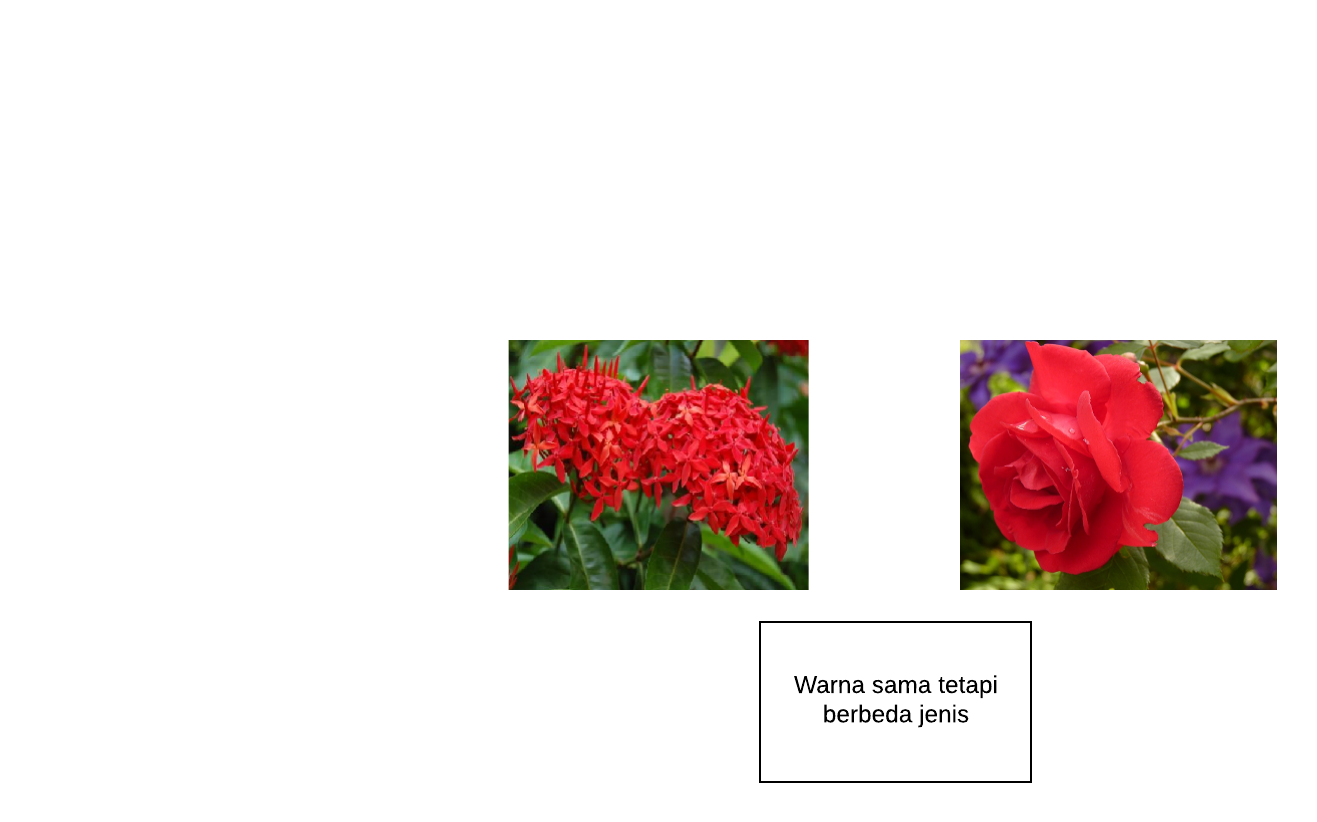
\includegraphics[scale=0.2]{figures/1174051/4/2.png}
\caption{contoh klasifikasi bunga}
\label{contoh}
\end{figure}

\item Jelaskan bagaimana teknik pembelajaran mesin pada teks pada kata-kata yang digunakan di youtube,jelaskan arti per atribut data csv dan sertakan ilustrasi buatan sendiri.\par
cara pembelajaran teks yang di gunakan youtube yaitu dengan cara merekam data yang sering di inputkan oleh user pada menu pencarian youtube. sehingga pada saat user akan mencari data yang serupa seringkali youtube menyediakan opsi atau rekomendasi-rekomendasi dari pencaharian. contoh saya menuliskan m maka muncul opsi pilihan master chep dan lainya yang berawalan m rekomendasi yang muncul merupakan kata-kata yang sering di cari oleh banyak user atau sering di buka oleh user itu sendiri.

\begin{figure}[ht]
\centering
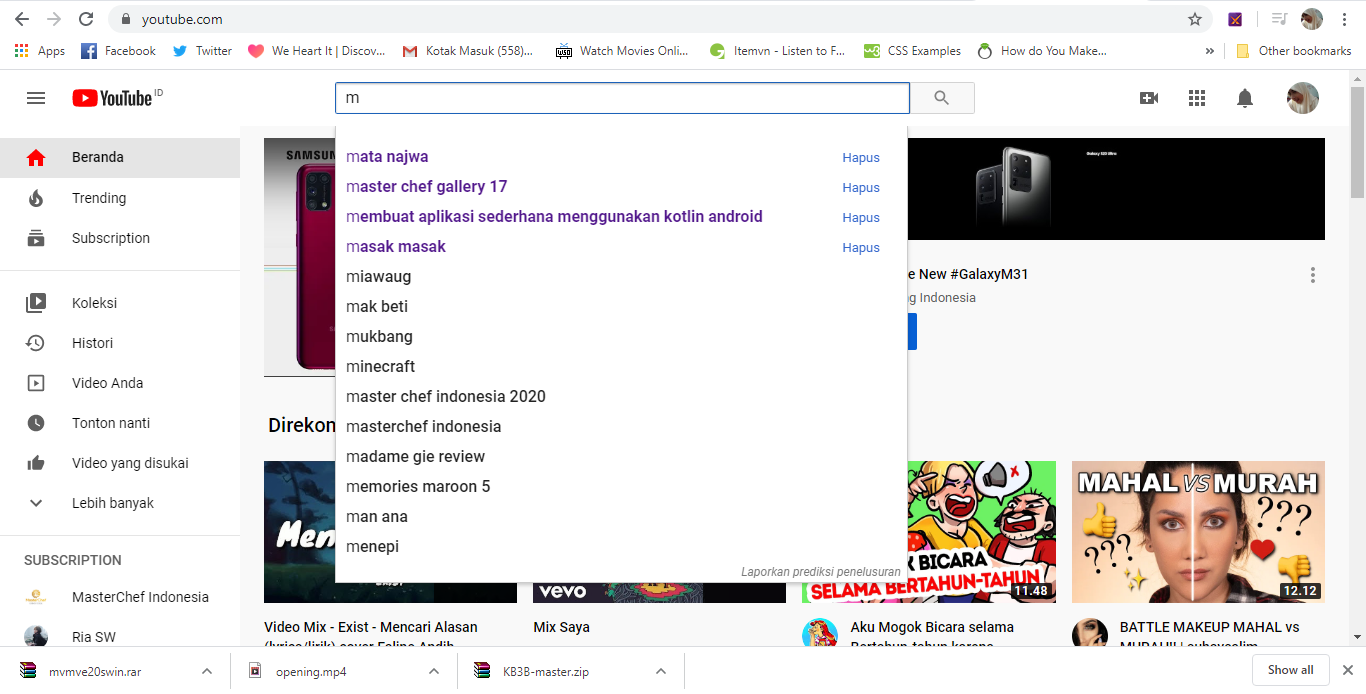
\includegraphics[scale=0.2]{figures/1174051/4/3.PNG}
\caption{contoh teknik pembelajaran mesin}
\label{contoh}
\end{figure}

\item Jelaskan apa yang dimaksud vektorisasi data.\par
vektorisasi data merupakan pemechan data menjadi bagian bagian yang lebih sederhana contoh pada satu paragraf terdiri dari 200 kata kemudian dilakukan vektorisasi dengancara membagi-bagi kata dalam paragraf tersebut ke dalam kalimat-kalimat yang terpisah kemudian di pecah lagi menjadi data dalam perkata selanjutnya kata kata tersebut di terjemahkan.

\item Jelaskan apa itu bag of words dengan kata-kata yang sederhana dan ilustrasi sendiri.
 bag of words merupakan peroses penyederhanaan kata-kata yang asalnya tersiri dalam satu kalimat atau satu paragraf di ubah menjadi perkata kemudian kata-kata tersebut di kumpulkan menjadi satu kelompok tanpa ada arti dari kata-kata yang telah di kumpulkan tersebut lalu di hitung frekuensi kemunculan dari kata tersebut.
 
\begin{figure}[ht]
\centering
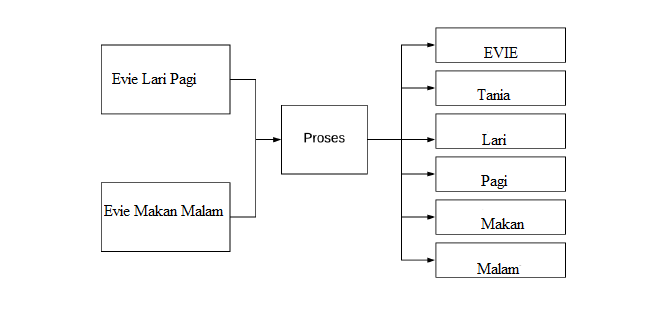
\includegraphics[scale=0.2]{figures/1174051/4/4.PNG}
\caption{contoh bag of words}
\label{contoh}
\end{figure}

\item Jelaskan apa itu TF-IDF, ilustrasikan dengan gambar sendiri.
 TF-IDF merupakan metode untuk menghitung bobot dari kata yang sering muncul pada suatu kalimat. metode ini menghitung nilai TF atau Term Frequency dan IDF atau Inverse Document Frequency pada setiap kata pada kalimat yang dijadikan acuan kata pada metode ini sering di sebut token adapun rumus dari metode ini.
 
\begin{figure}[ht]
\centering
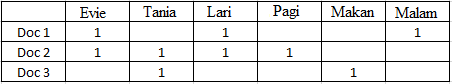
\includegraphics[scale=0.2]{figures/1174051/4/5.PNG}
\caption{contoh TF-IDF}
\label{contoh}
\end{figure}

\end{enumerate}


\subsection{Praktek}
\begin{enumerate}
    \item Buat aplikasi sederhana menggunakan pandas, buat data dummy format csv sebanyak 500 baris dan melakukan load ke dataframe pandas. Jelaskan arti setiap baris kode yang dibuat.
    \lstinputlisting[firstline=1, lastline=11]{src/1174051/4/praktek1.py}
    \item Dari dataframe tersebut, dipecah menjadi dua dataframe yaitu 450 row pertama dan 50 row sisanya(Harus beda dengan teman sekelas)
    \lstinputlisting[firstline=12]{src/1174051/4/praktek1.py}
    \item Praktekkan vektorisasi dan klasifikasi dari data Shakira dengan decision tree. Tunjukkan keluarannya dari komputer sendiri dan artikan maksud dari setiap luaran yang didapatkan.
    \lstinputlisting[firstline=8, lastline=49]{src/1174051/4/praktek3.py}
    \begin{figure}[ht]
        \centering
        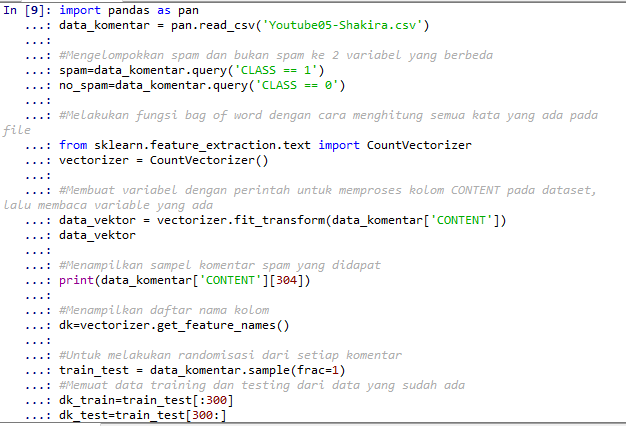
\includegraphics[scale=0.2]{figures/1174051/4/6.PNG}
        \caption{Melakukan vektorisasi dan mengambil salah satu contoh}
        \label{contoh6}
    \end{figure}
    \item Cobalah klasifikasikan dari data vektorisasi yang ditentukan di nomor sebelumnya dengan klasifikasi SVM. Tunjukkan keluarannya dari komputer sendiri dan artikan maksud setiap luaran yang didapatkan.
    \lstinputlisting[firstline=53, lastline=57]{src/1174051/4/praktek3.py}
    \begin{figure}[ht]
        \centering
        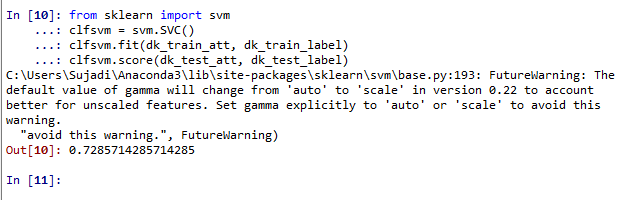
\includegraphics[scale=0.2]{figures/1174051/4/7.PNG}
        \caption{Melakukan prediksi CVM berdasarkan nilai}
        \label{contoh7}
    \end{figure}
    \item Coba klasifikasikan dari data vektorisasi yang ditentukan di nomor sebelumnya dengan klasifikasi Decision Tree. Tunjukkan kelaurannya dari komputer sendiri dan artikan maksud setiap luaran yang didapatkan.
    \lstinputlisting[firstline=60, lastline=64]{src/1174051/4/praktek3.py}
    \begin{figure}[ht]
        \centering
        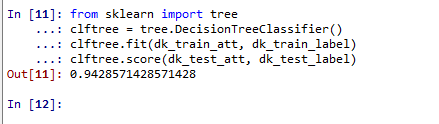
\includegraphics[scale=0.2]{figures/1174051/4/8.PNG}
        \caption{Klasifikasi data dari vektorisasi yang ada dengan decision tree}
        \label{contoh8}
    \end{figure}
    \item Plotlah confusion matrix dari praktek modul ini menggunakan matplotlib. Tunjukkan keluarannya dari komputer sendiri dan artikan maksud setiap luaran yang didapatkan
    \lstinputlisting[firstline=66, lastline=72]{src/1174051/4/praktek3.py}
    \begin{figure}[ht]
        \centering
        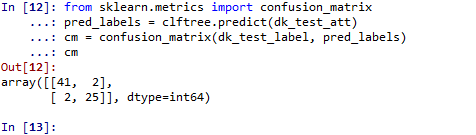
\includegraphics[scale=0.2]{figures/1174051/4/9.PNG}
        \caption{Penggunaan confusion matrix}
        \label{contoh9}
    \end{figure}
    \item Jalankan program cross validation pada bagian teori bab ini. Tunjukkan keluarannya dari komputer sendiri dan artikan mnaksud setiap luaran yang didapatkan.
    \lstinputlisting[firstline=74, lastline=90]{src/1174051/4/praktek3.py}
    \begin{figure}[ht]
        \centering
        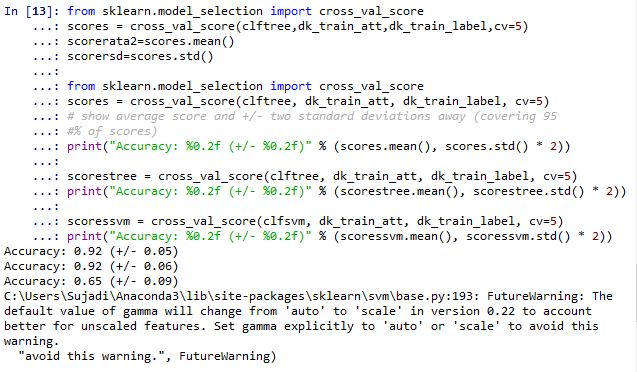
\includegraphics[scale=0.2]{figures/1174051/4/10.PNG}
        \caption{Mengambil tingkat akurasi dari klasifikasi data dan prediksi}
        \label{contoh11}
    \end{figure}
    \item Buatlah program pengamatan komponen informasi pada bagian teori bab ini. Tunjukkan keluarannya dari komputer sendiri dan artikan maksud setiap luaran yang didapatkan
    \lstinputlisting[firstline=91]{src/1174051/4/praktek3.py}
    \begin{figure}[ht]
        \centering
        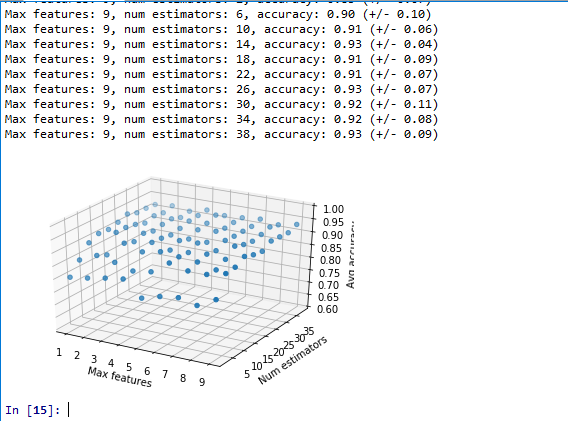
\includegraphics[scale=0.2]{figures/1174051/4/11.PNG}
        \caption{Melakukan regresi data dengan numpy dan mengambil fitur - fitur yang ada}
        \label{contoh12}
    \end{figure}
\end{enumerate}
\subsection{Penanganan Error}
\subsubsection{Sreenshoot Error}
\begin{enumerate}
\item Error 1
\begin{figure}[H]
\centering
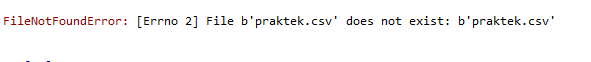
\includegraphics[scale=1]{figures/1174051/4/12.PNG}
\caption{error 1}
\label{error 1}
\end{figure}        
\end{enumerate} 
\subsubsection{Penanganan untuk Error}
\begin{enumerate}
\item penanganan 1, kesalahan pada nama file yang dituju, dimana cara penanganannya adalah memasukkan nama file dengan benar
\begin{figure}[H]
\centering
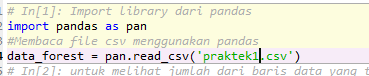
\includegraphics[scale=1]{figures/1174051/4/13.PNG}
\caption{penanganan1}
\label{penanganan1}
\end{figure}
\end{enumerate}